\documentclass{article}
\usepackage[utf8]{inputenc}
\usepackage{mathtools}
\usepackage{pgfplots}
\usepackage{natbib}
\usepackage{amsmath}
\usepackage{amssymb}
\usepackage{amsfonts}
\usepackage{natbib}
\usepackage{graphicx}
\usepackage{minted}
\usepackage{ dsfont }
\usepackage[a4paper,margin=1in,footskip=0.25in]{geometry}
\allowdisplaybreaks


\title{CSE546 Machine Learning HW2}
\author{Bobby Deng | 1663039 | dengy7 }
\date{3 May 2020}

\begin{document}
	\maketitle


\section*{A.0}

\subsection*{a. [2 points] Suppose that your estimated model for predicting house prices has a large positive weight on	’number of bathrooms’. Does it implies that if we remove the feature ”number of bathrooms” and refit	the model, the new predictions will be strictly worse than before? Why?}

Answer:  Yes, when there is a large positive weight comparatively to other weights. It means that feature is important and may have a strong positive linear relationship with the target class. 

\subsection*{b. [2 points] Compared to L2 norm penalty, explain why a L1 norm penalty is more likely to result in a larger number of 0s in the weight vector or not?}

Answer:  The gradient for l1 is always the same, however l2 norm produce a gradient with diminishing return as weights move to zero. If we remove that important feature it spread the effect to other features which produces more bias. So we want to keep important feature and remove less important features.


\subsection*{c. [2 points] In at most one sentence each, state one possible upside and one possible downside of using the following regularizer: $ (\sum_{i} |w_i|^{0.5}) $ }

Answer: The downside it this norm tends to choose bigger coefficients compared to L2 and might lead to over-fitting.One possible upside could be that it only produce positive gradient and may converge faster.

\subsection*{d. [1 points] True or False: If the step-size for gradient descent is too large, it may not converge.}

Answer: True

\subsection*{e. [2 points] In your own words, describe why SGD works.}

Answer: SGD refers to Stochastic Gradient Descent. And it is computing the gradients of one sample and update the weights. And do this process over and over again until some converge conditions are met.

\subsection*{f. [2 points] In at most one sentence each, state one possible advantage of SGD (stochastic gradient descent) over GD (gradient descent) and one possible disadvantage of SGD relative to GD.}

Answer: SGD might be a little bit computationally efficient. The disadvantage is that SGD produce unstable gradients and it is likely to bouncing back and forth.


\section*{A.1}

\subsection*{a.}
To prove it is a norm, we want to prove:
\[ ||x+y|| \le ||x|| + ||y||  \]

First:
\[ |a+b| -> |a+b|^2 = (a+b)^2 = a^2 + 2ab + b^2\]
\[ |a| + |b| -> (|a| + |b|)^2 = a^2 + 2|a||b| + b^2 \]
And $2|a||b| \ge 2ab$,
So:
\[ |a+b| \le |a| + |b| \]
Then from above we can get:
\[ \sum_{i=1}^{n}|a+b| \le \sum_{i=1}^{n}|a| + \sum_{i=1}^{n}|b| \]
So it satisfy the triangle inequality:
\[ ||a+b|| \le ||a|| + ||b||  \]
So it is a norm.

\subsection*{b.}
This is not a norm. For points x(1,4), y(4,1), it does not satisfy the triangle inequality. 

\section*{B.1}
\[ \sqrt{\sum_{i=1}^{n} x_i^2}  \le \sum_{i=1}^{n} |x_i|\]
\[ \sum_{i=1}^{n} x_i^2 \le (\sum_{i=1}^{n} |x_i|)^2 \]
Let $|x_i| = Z_i$
\[ \sum_{i=1}^{n} Z_i^2 \le  (\sum_{i=1}^{n} Z_i)^2\]
\[\sum_{i=1}^{n} Z_i^2 \le  (\sum_{j=1}^{n}Z_j) (\sum_{i=1}^{n} Z_i) \]
\[ \sum_{i=1}^{n} Z_i^2 \le (Z_1+Z_2+ \dots + Z_n) (Z_1+Z_2+ \dots + Z_n) \]
\[ \sum_{i=1}^{n} Z_i^2 \le  \sum_{i=1}^{n}Z_j^2 + \sum_{j=1}^{n} \sum_{j \ne i}^{n} Z_j Z_i\]
With this equality, we can conclude that with higher order, there will be more terms on the right side of the equation. So:
\[ ||x|| \infty \le ||x||_2 \le ||x||_1 \]


\section*{A.2}

\begin{itemize}
\item 1 is not convex, the line segment from b to c it not convex set.

\item 2 is convex, every points inside is convex set.

\item 3 is not convex, the line segment from a to d is not convex set.
\end{itemize}


\section*{A.3}

\begin{itemize}
\item a. Yes
\item b. No, the segment from a to c is not convex set.
\item c. No, the line segment from a to d is not convex set.
\item d. Yes
\end{itemize}


\section*{B.2}
\subsection*{a.}
The goal it to achieve triangle inequality that:
\[ f(ax + (1-a)y) \le af(x) + (1-a)f(y) \]
Firstly, lets compute the left part:
\[ f(ax + (1-a)y) = |ax + (1-a) y| \]
Assume:
\[ |ax + (1-a) y| \le a|x| + (1-a)|y| \]
Square left and right:
\[ a^2x^2 + 2a(1-a)xy + (1-a)^2y^2 \le a^2x^2 + 2a(1-a)|x||y| + (1-a)^2y^2\]
Since x and y could positive and negative so:
\[ 2a(1-a)xy \le  2a(1-a)|x||y| \]
So in fact the assumption is right:
\[ |ax + (1-a) y| \le a|x| + (1-a)|y| \]
So it is convex function.

\subsection*{b.}
The same as previous question, we need to prove the triangle inequality to show it is convex function.
\[ ||ax + (1-a)y|| \le a||x|| + (1-a)||y|| \le a + (1-a) = 1 \]
So from above, we proved that it satisfy the triangle inequality, and so it is convex function.

\subsection*{c.}
No, it is not convex function and we can see it from the graph that if we draw two points on the graph and it could be above the function area. So the set is not a convex set. \\

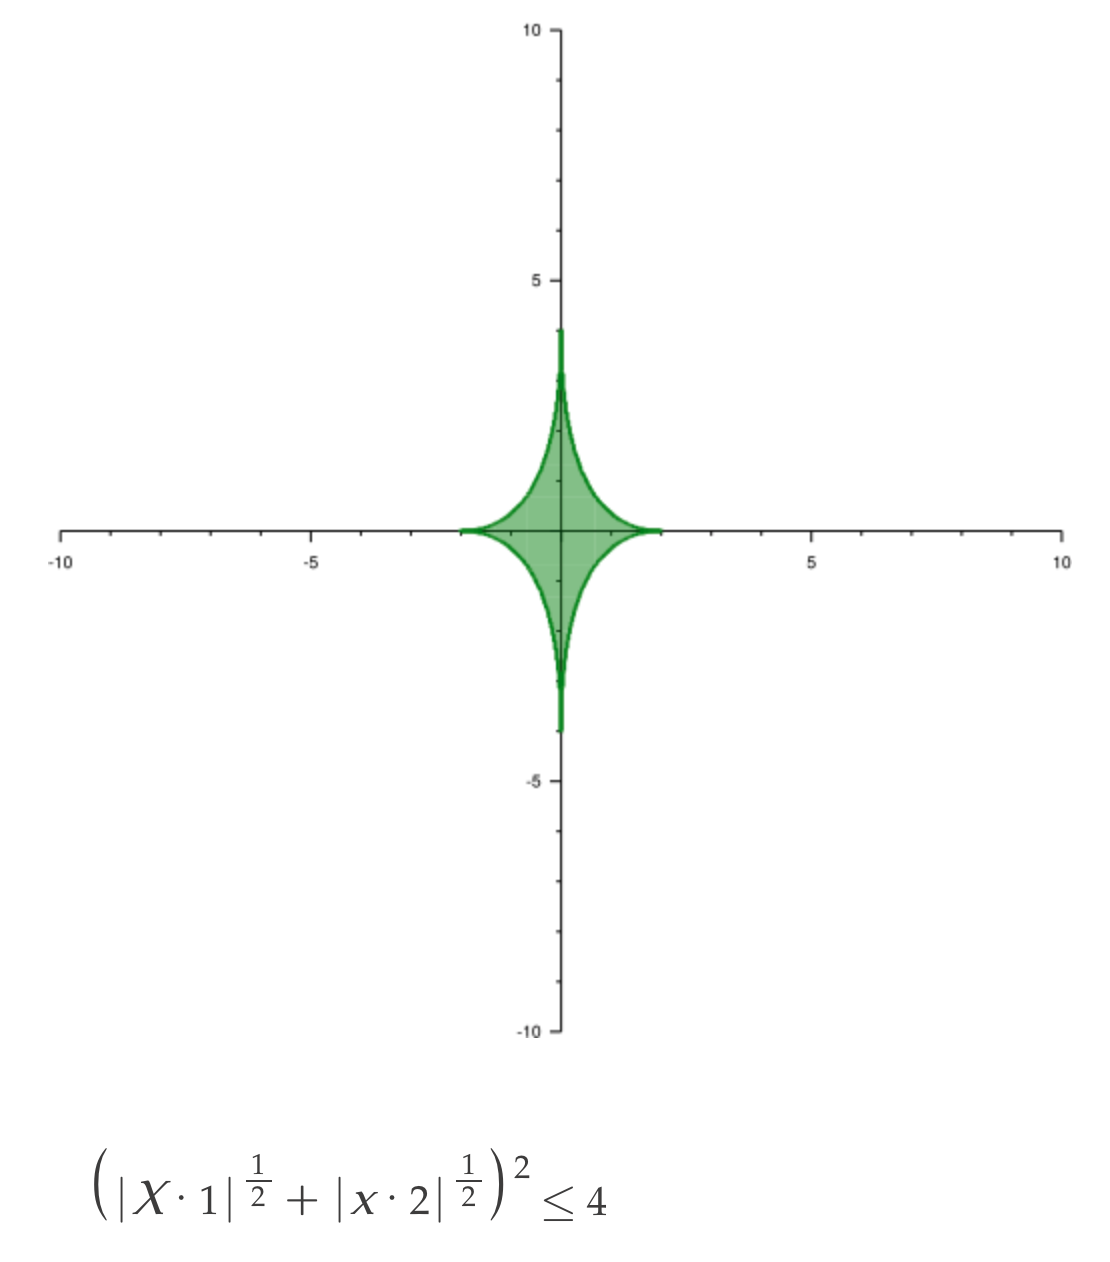
\includegraphics[width=10cm, height=7cm]{B2_c.png}



\section*{B.3}

\subsection*{a.}
We want to prove the triangle inequality: 
\[ f(ax_1 + (1-a)x_2) \le af(x_1) + (1-a)f(x-2) \]
Let:
\[ w_i = ax_i + (1-a)y_i \]
We know these two functions are convex function separately, now we compute 2 parts of the function separately:
\[ \sum_{i=1}^{n} \ell_i (w_i) \le a\sum_{i=1}^{n} \ell (x_i) + (1-a)\sum_{i=1}^{n} \ell (y_i) \]
\[ \sum_{i=1}^{n} \lambda ||w_i|| \le  a\sum_{i=1}^{n} \lambda ||x_i|| + (1-a)\sum_{i=1}^{n}\lambda||y_i|| \]
So, we combine the two equation into one:
\[ \sum_{i=1}^{n} \ell_i (w_i) +  \sum_{i=1}^{n} \lambda ||w_i|| \le a\sum_{i=1}^{n} \ell (x_i) + (1-a)\sum_{i=1}^{n} \ell (y_i) + a\sum_{i=1}^{n} \lambda ||x_i|| + (1-a)\sum_{i=1}^{n}\lambda||y_i|| \]
Move terms around:
\[ \sum_{i=1}^{n} \ell_i (w_i) +  \sum_{i=1}^{n} \lambda ||w_i|| \le a\sum_{i=1}^{n} \ell (x_i) + a\sum_{i=1}^{n} \lambda ||x_i|| + (1-a)\sum_{i=1}^{n} \ell (y_i) + (1-a)\sum_{i=1}^{n}\lambda||y_i|| \]
Simplify and we get the triangle inequality:
\[ \sum_{i=1}^{n} \ell_i (w_i) +  \sum_{i=1}^{n} \lambda ||w_i|| \le a\sum_{i=1}^{n} \Big( \ell (x_i) + \lambda ||x_i|| \Big) + (1-a)\sum_{i=1}^{n} \Big(  \ell (y_i) + \lambda||y_i|| \Big) \]
So, the sum of the two convex function is still a convex function.


\subsection*{b.}
We could easily find the local minimum in convex function and in convex function local minimum is global minimum.


\section*{A.4}
\begin{minted}[mathescape,linenos,obeytabs=true,tabsize=2]{python}
import numpy as np
import matplotlib.pyplot as plt
import pandas as pd

def generate_x(n,d):
	return np.random.standard_normal((n,d))

def generate_y(n, d, k, X):
	w = np.zeros((d,1))
	for i in range(0, d):
		if (0 <= i and i < k): 
			w[i] = (i + 1)/k
		else:
			w[i] = 0

	y = np.zeros((n, 1))
	for i in range(n):
		y[i] = w.T @ X[i] + np.random.standard_normal()
	return y, w


def compute_initial_lamb(x, y):
	n, d = x.shape
	lamb_array = np.zeros((d, 1))
	for k in range(d):
		lamb_temp = 2 * abs(x[:, k].T @ (y - np.mean(y)))
		lamb_array[k] = lamb_temp
	return max(lamb_array)

class Lasso:
	
	def __init__(self, lamb=0.001, delta=0.05):
		self.lamb = lamb
		self.last_w = None
		self.b = 0.0
		self.delta = delta
		self.loss_list = []
		self.last_selected_coef = []
		self.selected_feature_index = [1, 3, 5, 7, 12]
	
	def coordinate_descent(self, X, y, initial_w):
		n, d = X.shape
		W = initial_w
		a = 2 * np.sum(np.power(X, 2), axis=0)  
		
		not_converge = True
		while not converged:
			self.b = np.average(y - X.dot(W))
			loss_prev = loss
			prev_w = np.copy(W)  
			for k in range(d):
				X_k = X[:, k]
				prev_wk = np.copy(W[k])
				W[k] = 0
				c_k = np.dot((y - (self.b * np.ones((n, 1)) + X.dot(W))).T, X_k)
				if 2 * c_k + self.lamb < 0:
					W[k] = (c_k * 2 + self.lamb) / a[k]
				elif 2 * c_k - self.lamb > 0:
					W[k] = (c_k * 2 - self.lamb) / a[k]
				else:
					W[k] = 0
			
			if sum(abs(W - prev_w)) <= sum(abs(self.delta * prev_w)):
				not_converge = False
				print(W)
			
			loss = np.sum(np.power((self.b * np.ones((n, 1)) + X.dot(W) - y), 2)) + self.lamb * np.sum(abs(W))
			self.loss_list.append(loss)
			self.last_w = W
			self.last_selected_coef = self.last_w.T[0][self.selected_feature_index]
	
	def predict(self, X):
	return X.dot(self.last_w)

\end{minted}




\subsection*{a.}

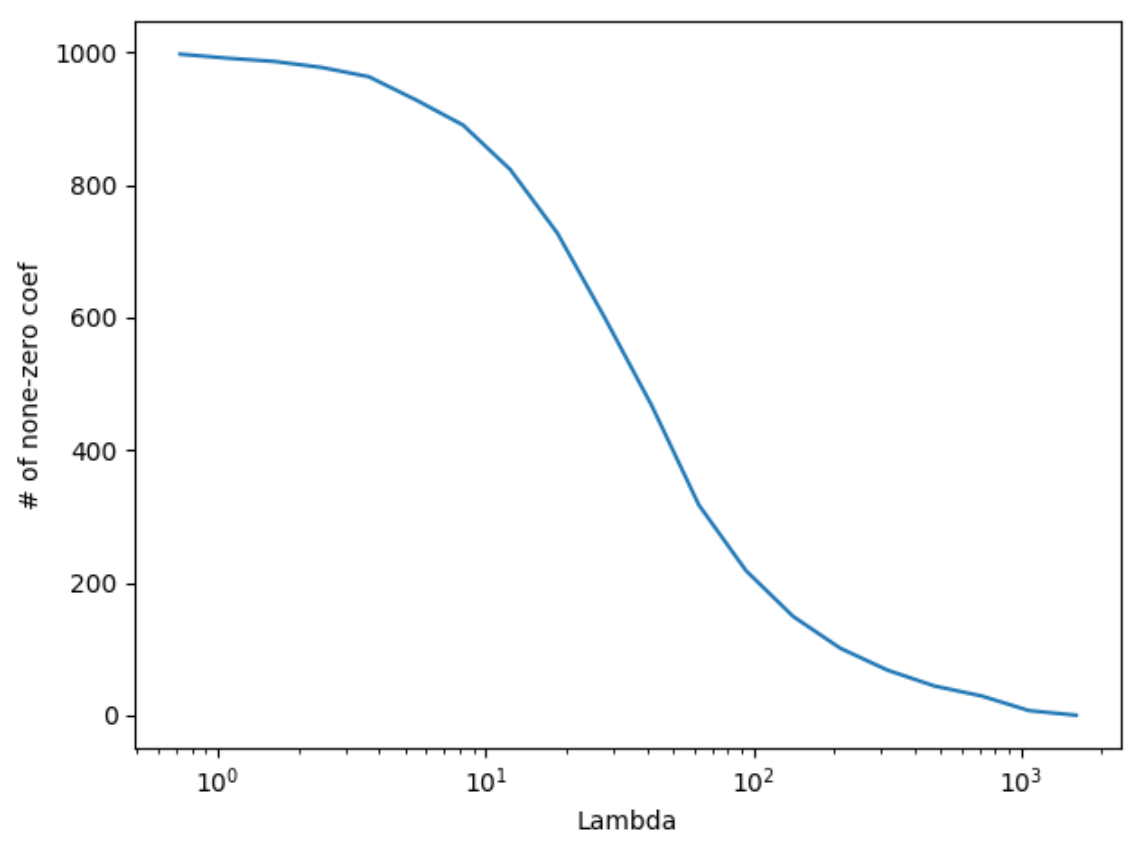
\includegraphics[width=10cm, height=7cm]{A4_a.png}


\begin{minted}[mathescape,linenos,obeytabs=true,tabsize=2]{python}
from A4_A5_starter import *

if __name__ == '__main__':
	n = 500
	d = 1000
	k = 100
	
	X_train = generate_x(n, d)
	y_train, W_init = generate_y(n, d, k, X_train)
	lam = compute_initial_lamb(X_train, y_train)
	number_of_nonezero_feature = []
	FDR_list = []
	TPR_list = []
	
	lam_list = lam * (1/1.5) ** np.arange(0, 20)
	
	for lam in lam_list:
		
		print("lam", lam)
		lasso = Lasso(lam, delta=0.4)
		lasso.coordinate_descent(X_train, y_train, np.zeros((d,1)))
		last_w = lasso.last_w.copy()
		print("Number of coe > 0:", sum(abs(last_w) > 0))
		number_nonezero = sum(last_w != 0)
		number_of_nonezero_feature.append(number_nonezero)
		
		
	plt.plot(lam_list, number_of_nonezero_feature)
	plt.xscale('log')
	plt.xlabel("Lambda")
	plt.ylabel("# of none-zero coef")
	plt.show()


\end{minted}




\subsection*{b.}


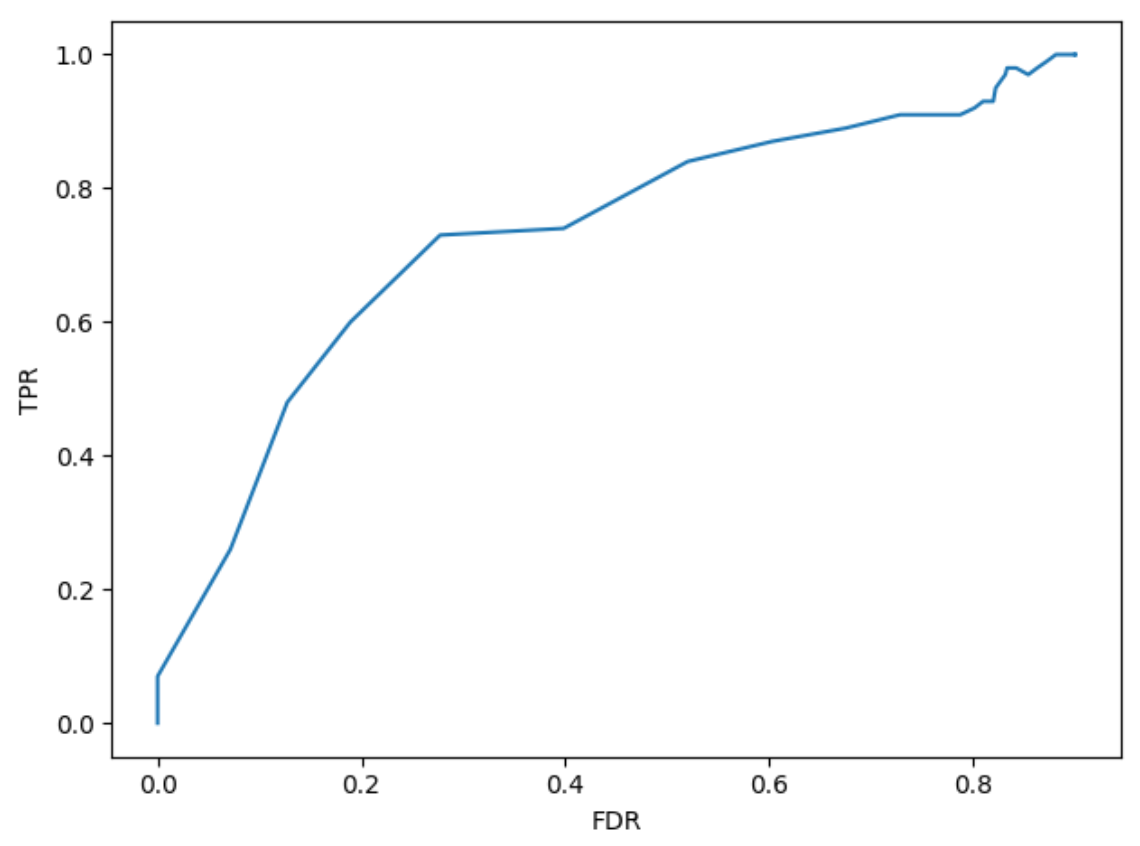
\includegraphics[width=10cm, height=7cm]{A4_b.png}


\begin{minted}[mathescape,linenos,obeytabs=true,tabsize=2]{python}
from A4_A5_starter import *

if __name__ == '__main__':
	n = 500
	d = 1000
	k = 100
	
	X_train = generate_x(n, d)
	y_train, W_init = generate_y(n, d, k, X_train)
	lam = compute_initial_lamb(X_train, y_train)[0]
	number_of_nonezero_feature = []
	FDR_list = []
	TPR_list = []
	
	lam_list = lam * (1/1.5) ** np.arange(0, 40)
	
	for lam in lam_list:
	
		print("lam", lam)
		lasso = Lasso(lam, delta=0.001)
		lasso.coordinate_descent(X_train, y_train, np.zeros((d,1)))
		last_w = lasso.last_w
		print("Number of coe > 0:", sum(abs(last_w) > 0))
		number_nonezero = sum(last_w != 0)
		number_of_nonezero_feature.append(number_nonezero)
		
		incorrect_none_zero = sum(last_w[W_init == 0] != 0)
		number_correct_none_zero = sum(last_w[W_init != 0] != 0)
		if incorrect_none_zero == 0:
			FDR = 0
			FDR_list.append(0)
		else:
			FDR = incorrect_none_zero / number_nonezero
			FDR_list.append(FDR)
		TPR = number_correct_none_zero / k
		TPR_list.append(TPR)
		
		print("FDR: ", FDR, " TPR: ", TPR)
	
	
	
	plt.plot(FDR_list, TPR_list)
	plt.xlabel("FDR")
	plt.ylabel("TPR")
	plt.show()

\end{minted}


\subsection*{c.}

When lambda gets bigger, number of none-zero term decrease until 0. When lambda is small enough, there is no zero term. I can see that it is important to chooes an proper lambda.


In the TPR-FDR relationship plot, they tends to have a positive relationship. When lambda is at max, all feature coeff are 0, so TPR and FDR are both 0. When lambda decrease, TPR and FDR both increase.

\section*{A.5}

\subsection*{a.}
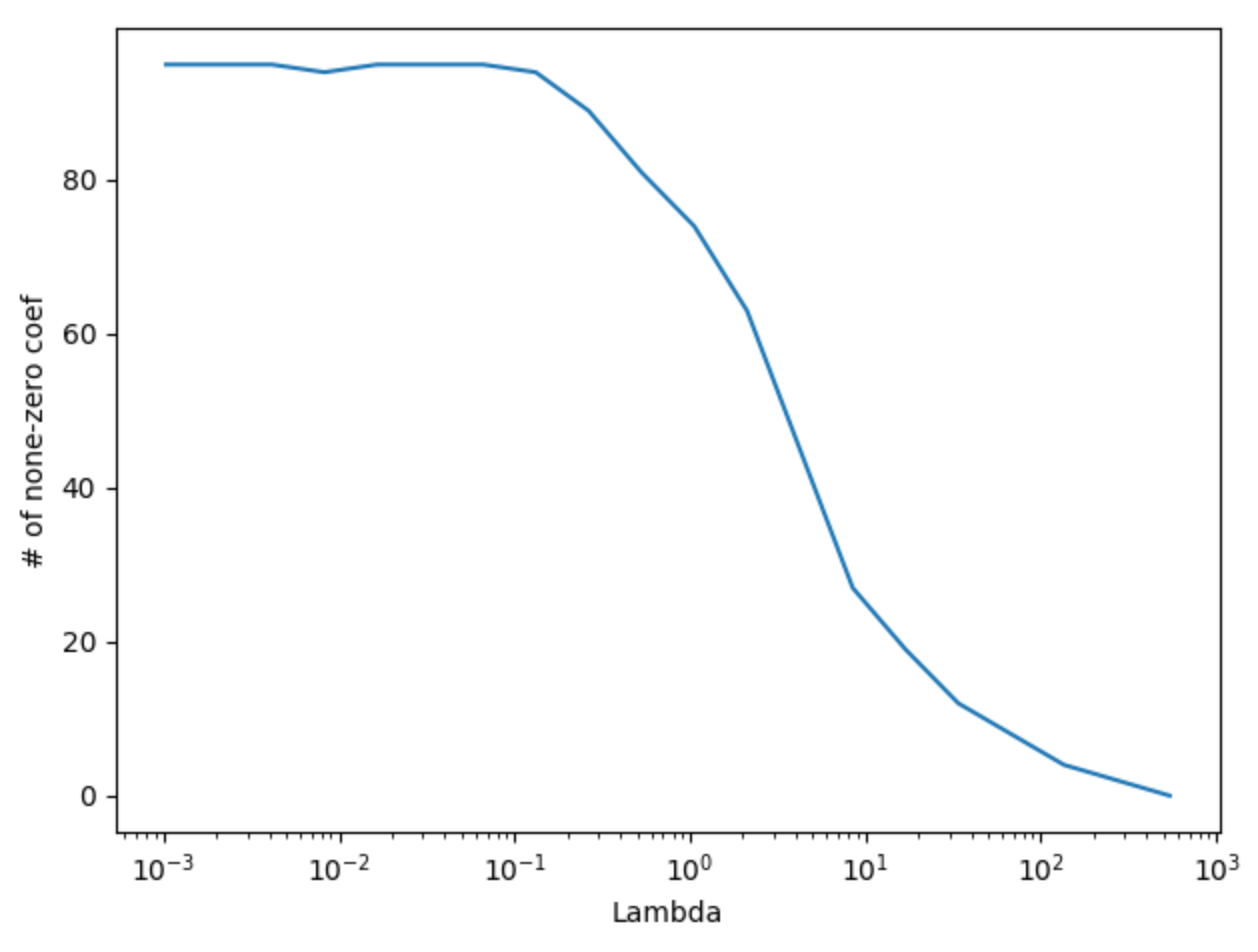
\includegraphics[width=10cm, height=7cm]{A5_a.png}

\subsection*{b.}
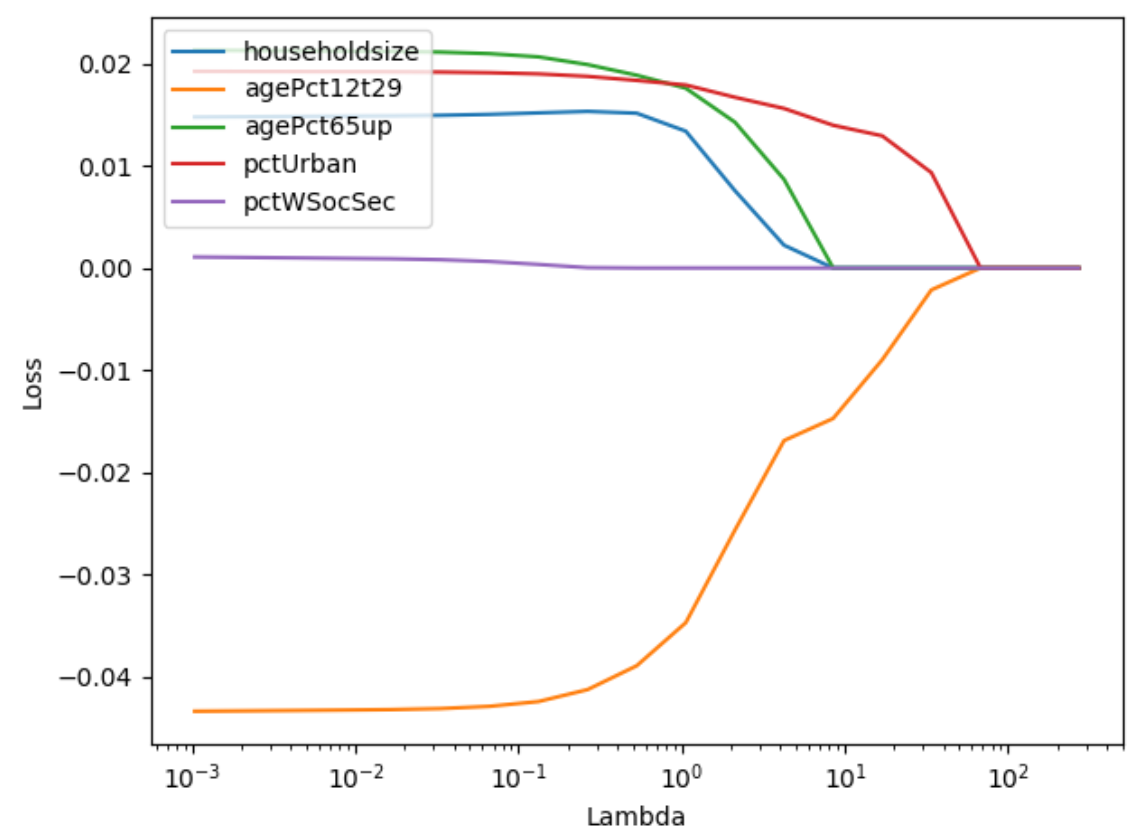
\includegraphics[width=10cm, height=7cm]{A5_b.png}

\subsection*{c.}
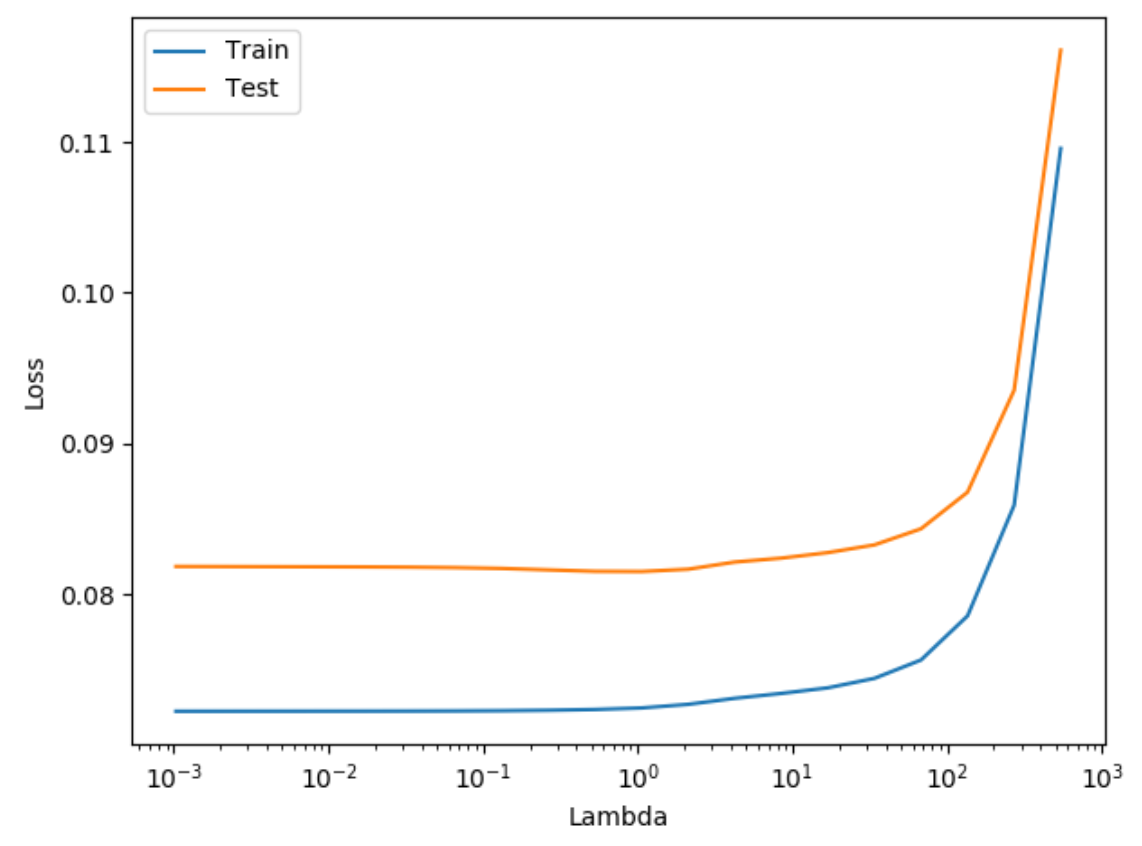
\includegraphics[width=10cm, height=7cm]{A5_c.png}

\subsection*{d.}

\begin{itemize}
\item      Coeff                   Name
\item   0.068025             PctIlleg

\item -0.070175          PctKids2Par

\item For highest positive feature: PctIlleg(percentage of kids born to never married (numeric - decimal)). A reasonable explanation for this is that in poor area people had less sense of contraception, can lead to unwanted kids burn. Also may become one of the reason. And poor districts may have higher crime rate as well.
\item For highest negative feature: PctKids2Par( percentage of kids in family housing with two parents (numeric - decimal)). This is really reasonable. With two parents probabaly means a good family, and higher such rate means the district are more good families. And this district might be rich and well educated and has good measure for preventing crime to take place.

\end{itemize}



\subsection*{e.}
This does not make sense, because mathematically, when where are more older people, a lot of other things will change as well. Meaning coefficients of other variable may change and then the model would not be the same. Then the crime rate may not decrease. On the other hand, crime is not produced by older people. It does not make sense to introduce more older people just in order to lower the crime rate. We should focused on what caused crime and reduce that factor.

\begin{minted}[mathescape,linenos,obeytabs=true,tabsize=2]{python}
import pandas as pd
import numpy as np
import matplotlib.pyplot as plt


class Lasso:

	def __init__(self, lamb=0.001, delta=0.05):
		self.lamb = lamb
		self.last_w = None
		self.b = 0.0
		self.delta = delta
		self.loss_list = []
		self.last_selected_coef = []
		self.selected_feature_index = [1, 3, 5, 7, 12]
	
	def coordinate_descent(self, X, y, initial_w):
		n, d = X.shape
		W = initial_w
		a = 2 * np.sum(np.power(X, 2), axis=0)  
		loss = np.sum(np.power((self.b * np.ones((n, 1)) + X.dot(W) - y), 2)) +
		 self.lamb * np.sum(abs(W))
		
		not_converge = True
		while not_converge:
			self.b = np.average(y - X.dot(W))
			loss_prev = loss
			prev_w = np.copy(W)  
			for k in range(d):
				X_k = X[:, k]

				W[k] = 0
				c_k = np.dot((y - (self.b * np.ones((n, 1)) + X.dot(W))).T, X_k)
				if 2 * c_k + self.lamb < 0:
					W[k] = (c_k * 2 + self.lamb) / a[k]
				elif 2 * c_k - self.lamb > 0:
					W[k] = (c_k * 2 - self.lamb) / a[k]
				else:
					W[k] = 0

			if sum(abs(W - prev_w)) <= sum(abs(self.delta * prev_w)):
				not_converge = False
				print(W)

			loss = np.sum(np.power((self.b * np.ones((n, 1)) + X.dot(W) - y), 2)) + self.lamb * np.sum(abs(W))
			self.loss_list.append(loss)
			self.last_w = W
			self.last_selected_coef = self.last_w.T[0][self.selected_feature_index]
			
	def predict(self, X):
		return X.dot(self.last_w)


def compute_initial_lamb(x, y):
	n, d = x.shape
	lamb_array = np.zeros((d, 1))
	for k in range(d):
		lamb_temp = 2 * abs(x[:, k].T @ (y - np.mean(y)))
		lamb_array[k] = lamb_temp
	return max(lamb_array)

if __name__ == "__main__":
	df_train = pd.read_table("crime-train.txt")
	df_test = pd.read_table("crime-test.txt")
	y_train = df_train["ViolentCrimesPerPop"].values.reshape(df_train.shape[0], 1)
	x_train = df_train.drop("ViolentCrimesPerPop", axis=1).values
	x_test = df_test.drop("ViolentCrimesPerPop", axis=1).values
	y_test = df_test["ViolentCrimesPerPop"].values.reshape(df_test.shape[0], 1)
	
	
	n ,d = x_train.shape
	lambda_max = compute_initial_lamb(x_train, y_train)
	initial_model = Lasso(lambda_max)
	initial_model.coordinate_descent(x_train, y_train, np.zeros((d, 1)))
	initial_w = initial_model.last_w
	
	lam_list = (lambda_max) * (1 / 2) ** np.arange(0, 20)
	householdsize_list = []
	agePct12t29_list = []
	agePct65up_list = []
	pctUrban_list = []
	pctWSocSec_list = []
	trained_w = []
	initial_loss_train = np.mean((initial_model.predict(x_train) - y_train)**2)
	initial_loss_test = np.mean((initial_model.predict(x_test) - y_test)**2)
	
	loss_train_list = [initial_loss_train]
	loss_test_list = [initial_loss_test]
	number_of_nonezero_feature = []
	
	# lam_list = [30,30]
	for lam in lam_list[1:]:
		model = Lasso(lam)
		model.coordinate_descent(x_train, y_train, initial_w)
		w_new = model.last_w.copy()
		number_of_nonezero_feature.append(np.count_nonzero(w_new))
		householdsize_list.append(w_new[1])
		agePct12t29_list.append(w_new[3])
		agePct65up_list.append(w_new[5])
		pctUrban_list.append(w_new[7])
		pctWSocSec_list.append(w_new[12])
		
		loss_train = np.mean((model.predict(x_train) - y_train)**2)
		loss_train_list.append(loss_train)
		loss_test = np.mean((model.predict(x_test) - y_test)**2)
		loss_test_list.append(loss_test)
	
	selected_coef_history = [householdsize_list, agePct12t29_list, 
	agePct65up_list, pctUrban_list, pctWSocSec_list]
	
	# A.5 a
	# Plot lambda against number_of_nonezero_feature
	plt.plot(lam_list[1:], number_of_nonezero_feature)
	plt.xscale('log')
	plt.xlabel("Lambda")
	plt.ylabel("# of none-zero coef")
	plt.show()
	
	# A.5 b
	# plot 5 different feature change with different lambda
	features = ['householdsize', 'agePct12t29', 'agePct65up', 'pctUrban', 'pctWSocSec']
	for i, feature in enumerate(features):
		plt.plot(lam_list[1:], selected_coef_history[i], label=feature)
		plt.xscale('log')
		plt.xlabel("Lambda")
		plt.ylabel("Loss")
		plt.legend(loc="upper left")
	plt.show()
	
	# A.5 c
	plt.plot(lam_list, loss_train_list, label="Train")
	plt.plot(lam_list, loss_test_list, label="Test")
	plt.xscale('log')
	plt.xlabel("Lambda")
	plt.ylabel("Loss")
	plt.legend(loc="upper left")
	plt.show()
	
	coeff_data = pd.DataFrame({"Coeff": (list(w_new.T[0])),
	"Name": df_train.columns[1:]}).sort_values(["Coeff"], ascending=False)
	coeff_data[:10]
	coeff_data[-10:]

\end{minted}

\section*{A.6}
\subsection*{a.}

We know:
\[ \mu_i(w, b) = \frac{1}{1 + exp(-y_i(b + x_i^Tw))} \]
Rewrite the above equiation:
\[ 1 + exp(-y_i(b + x_i^Tw)) = \frac{1}{\mu_i(w, b)} \]
\[  exp(-y_i(b + x_i^Tw)) = \frac{1}{\mu_i(w, b)} - 1 \]
\[ exp(-y_i(b + x_i^Tw)) = \frac{1}{\mu_i(w, b)} - \frac{\mu_i(w, b)}{\mu_i(w, b)} \]
\[ exp(-y_i(b + x_i^Tw)) = \frac{ 1 - \mu_i(w, b)}{\mu_i(w, b)} \]
Now we have: $exp(-y_i(b + x_i^Tw)) = \frac{ 1 - \mu_i(w, b)}{\mu_i(w, b)}$
Then we compute gradient of L2 logistic regression: \newline
To derive the gradient of w:
\[ \nabla_w J(w, b) = \frac{1}{n} \sum_{i=1}^{n} \frac{exp(-y_i(b + x_i^Tw))}{1 + exp(-y_i(b + x_i^Tw))} * (-y_ix_i^T) + 2 \lambda w \]
\[ = \frac{1}{n} \sum_{i=1}^{n} \frac{1 - \mu_i(w, b)}{\mu_i(w, b)} * \mu_i(w, b) * (-y_ix_i^T) + 2 \lambda w \]
\[ = \frac{1}{n} \sum_{i=1}^{n} \big(1 - \mu_i(w, b)\big) * (-y_ix_i^T) + 2\lambda w \]
To derive the gradient of b:
\[ \nabla_b J(w, b) \frac{1}{n} \sum_{i=1}^{n} \frac{exp(-y_i(b + x_i^Tw))}{1 + exp(-y_i(b + x_i^Tw))} * (-y_i) \]
\[ = \frac{1}{n} \sum_{i=1}^{n} \frac{1 - \mu_i(w, b)}{\mu_i(w, b)} * \mu_i(w, b) * (-y_i)\]
\[  \frac{1}{n} \sum_{i=1}^{n} \Big( 1 - \mu_i(w, b) \Big) * (-y_i) \]


\subsection*{b.}
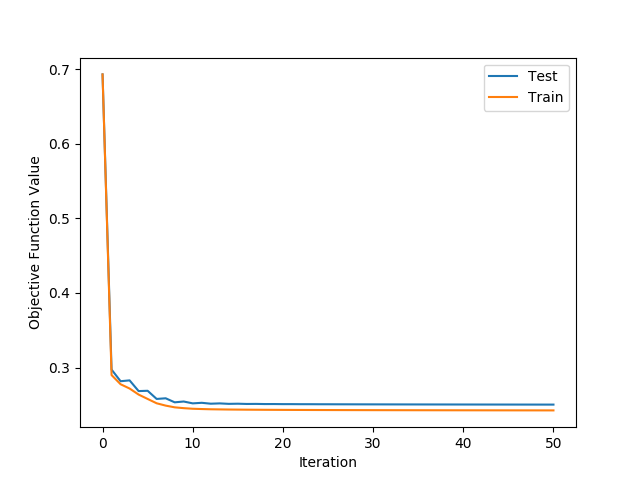
\includegraphics[width=9cm, height=6cm]{A6_b_1.png}
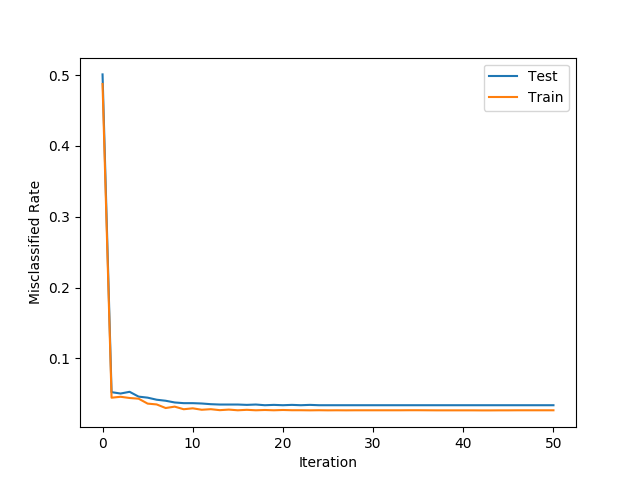
\includegraphics[width=9cm, height=6cm]{A6_b_2.png}

\subsection*{c.}
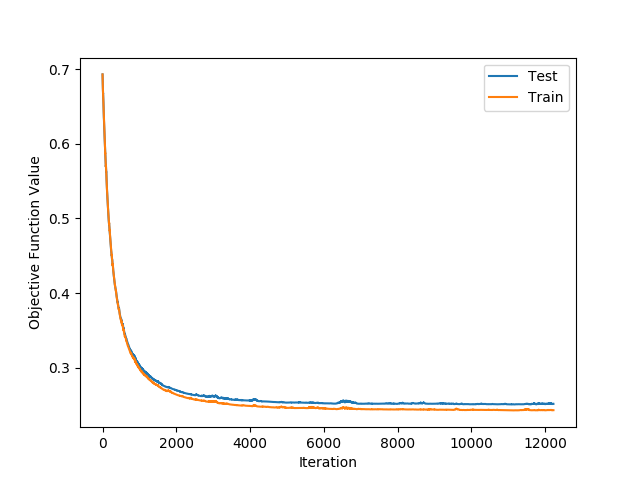
\includegraphics[width=9cm, height=6cm]{A6_c_1.png}
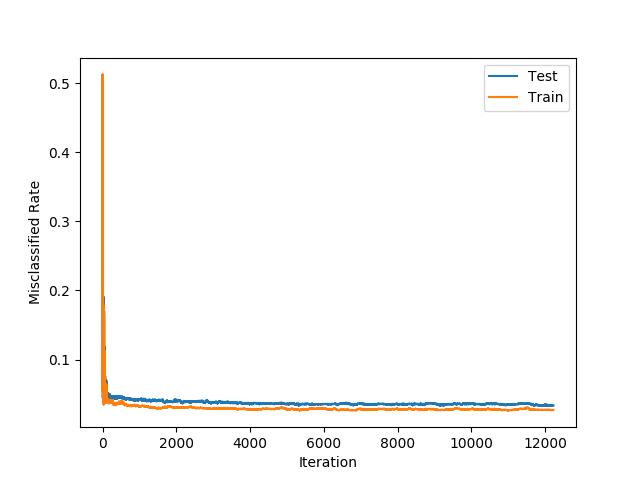
\includegraphics[width=9cm, height=6cm]{A6_c_2.png}

\subsection*{d.}
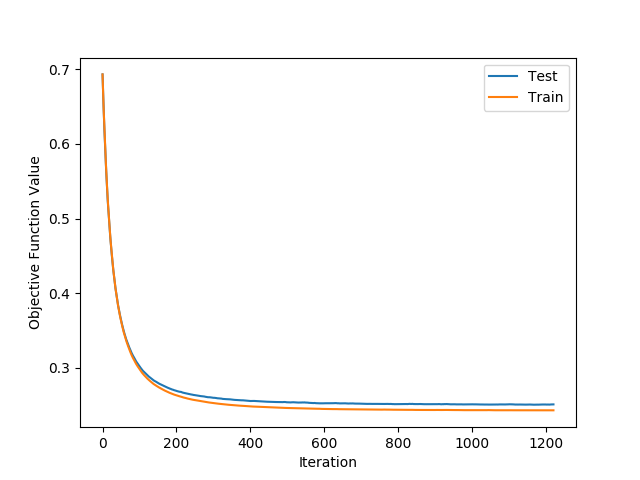
\includegraphics[width=9cm, height=6cm]{A6_d_1.png}
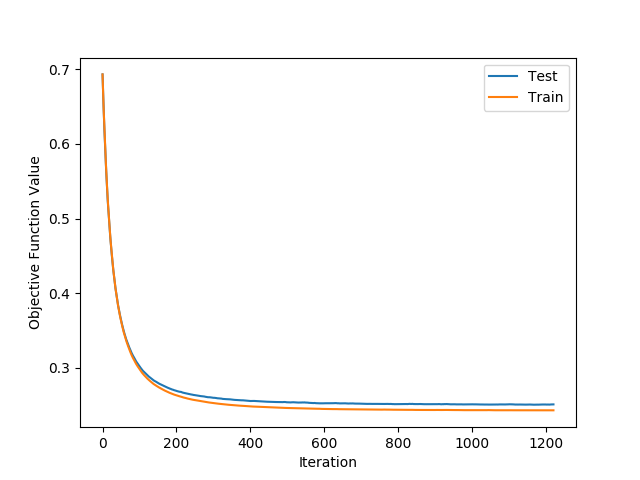
\includegraphics[width=9cm, height=6cm]{A6_d_1.png}

\begin{minted}[mathescape,linenos,obeytabs=true,tabsize=2]{python}
import numpy as np
import scipy.linalg as la
import matplotlib.pyplot as plt
from mnist import MNIST

np.random.seed(666)
lam = 0.1


def load_data():
	mndata = MNIST('python-mnist/data/')
	X_train, labels_train = map(np.array, mndata.load_training())
	X_test, labels_test = map(np.array, mndata.load_testing())
	X_train = X_train / 255.0
	X_test = X_test / 255.0
	
	labels_train = labels_train.astype(np.int16)
	labels_test = labels_test.astype(np.int16)
	X_train = np.vstack( (X_train[labels_train == 2], X_train[labels_train == 7]))
	y_train = np.hstack((labels_train[labels_train == 2], labels_train[labels_train == 7]))
	y_train[y_train == 2] = -1
	y_train[y_train == 7] = 1
	
	X_test = np.vstack((X_test[labels_test == 2], X_test[labels_test == 7]))
	y_test = np.hstack((labels_test[labels_test == 2], labels_test[labels_test == 7]))
	y_test[y_test == 2] = -1
	y_test[y_test == 7] = 1
	
	print(X_train.shape, y_train.shape, y_train.sum())
	return (X_train, y_train, X_test, y_test)


def descent(X, Y, w, b, learning_rate=0.01):

	u = 1.0 / (1.0 + np.exp(-Y * (b + X.dot(w))))
	gradient_b = (-Y * (1 - u)).mean()
	b -= learning_rate * gradient_b
	
	u = 1.0 / (1.0 + np.exp(-Y * (b + X.dot(w))))
	xy = np.multiply(X.T, Y)
	gradient_w = (- xy * (1 - u)).mean(axis=1) + 2 * lam * w
	w -= learning_rate * gradient_w
	
	return (w, b)


def objective_function_value(X, Y, w, b):
	log_error = np.log(1.0 + np.exp(-Y * (b + X.dot(w))))
	obj_value = log_error.mean() + L * np.linalg.norm(w, 2)
	
	predicted = b + X.dot(w)
	predicted[predicted < 0] = -1
	predicted[predicted >= 0] = 1
	correct = np.sum(predicted == Y)

	error = 1.0 - float(correct) / float(X.shape[0])
	
	return (obj_value, error)


def binary_logistic_regression(X_train, Y_train, X_test, Y_test, learning_rate, 
epochs, batch=0, save_plt_name="A6"):
	n, d = X_train.shape
	w = np.zeros(d)
	b = 0
	
	iterations = []
	test_objective_list = []
	train_objective_list = []
	test_error_list = []
	train_error_list = []
	obj_train, error = objective_function_value(X_train, Y_train, w, b)
	test_obj, test_error = objective_function_value(X_test, Y_test, w, b)
	test_objective_list.append(test_obj)
	train_objective_list.append(obj_train)
	test_error_list.append(test_error)
	train_error_list.append(error)
	iterations.append(0)
	
	i = 1
	for epoch in range(epochs):
		n, d = X_train.shape
		ramdom_index = np.random.permutation(n) 
		X_train = X_train[ramdom_index]
		Y_train = Y_train[ramdom_index]
		X_list = np.array_split(X_train, n / batch)
		Y_list = np.array_split(Y_train, n / batch)
		

		for X_split, Y_split in zip(X_list, Y_list):
			w, b = descent(X_split, Y_split, w, b, learning_rate)
			obj_train, error = objective_function_value(X_train, Y_train, w, b)
			obj_test, test_error = objective_function_value(X_test, Y_test, w, b)
			
			test_objective_list.append(obj_test)
			train_objective_list.append(obj_train)
			test_error_list.append(test_error)
			train_error_list.append(error)
			iterations.append(i)
			i += 1
	
	plt.plot(iterations, test_objective_list, label="Test")
	plt.plot(iterations, train_objective_list, label="Train")
	plt.xlabel("Iteration")
	plt.ylabel("Objective Function Value")
	plt.legend()
	plt.savefig("/Users/yinruideng/Desktop/senior_spring/cse546/hw/hw2/latex/"+ 
	save_plt_name + "_1.png")
	plt.show()
	
	plt.plot(iterations, test_error_list, label="Test")
	plt.plot(iterations, train_error_list, label="Train")
	plt.xlabel("Iteration")
	plt.ylabel("Misclassified Rate")
	plt.legend()
	plt.savefig("/Users/yinruideng/Desktop/senior_spring/cse546/hw/hw2/latex/"+ 
	save_plt_name + "_2.png")
	plt.show()

if __name__ == '__main__':
	X_train, Y_train, X_test, Y_test = load_data()
	n, d = X_train.shape
	print("#######  Gradient Descent #######")
	binary_logistic_regression(X_train, Y_train, X_test, Y_test, 0.5, 50, batch=n, 
	save_plt_name="A6_b")
	print("#######  Stochastic Gradient Descent  #######")
	binary_logistic_regression( X_train, Y_train, X_test, Y_test, 0.001, 1, batch=1, 
	save_plt_name="A6_c")
	print("#######  Mini Batch Gradient Descent  #######")
	binary_logistic_regression( X_train, Y_train, X_test, Y_test, 0.01, 10, batch=100, 
	save_plt_name="A6_d")

\end{minted}

\section*{B.4}
\subsection*{a.}
In this problem, in order to compute the gradient vector of the weights, we could compute individual gradient separately and then put them into an vector.

From the question we can rewrite the gradient equation and add softmax to it.
\[ \nabla_w \mathcal{L}(W) = - \sum_{i=1}^{n} x_i (y_i - \frac{exp(W^Tx_i)}{\sum_{j=i}^{k} exp(W^Tx_i)})^T \]

To prove the above equation, we compute the gradients individually:
\[ \mathcal{L}(W) = - \sum_{i=1}^{n} \sum_{\ell = i}^{k} \mathds{1}   \{y_i  = \ell\} log(\frac{exp(W^Tx_i)}{\sum_{j=i}^{k} exp(W^Tx_i)}) \]

\[ \nabla_w^t \mathcal{L}(W) = - \sum_{i=1}^{n}  \nabla_w^t \Big(  \mathds{1}   \{y_i  = t\} log(\frac{exp(W^Tx_i)}{\sum_{j=i}^{k} exp(W^Tx_i)})  \Big) \]
Then we take derivative, and note the following because derivative other than $w^j = w^t$ equals to 0: 
\[ \frac{\partial(\sum_{j=1}^{k} exp(w^{(j)} x_i)))}{\partial w^t} = exp(w^{(t)} x_i)) x_i\]
Then with this in mind:


\[ \nabla_{w^t} \mathcal{L}(W) = - \sum_{i=1}^{n}  \Big(  \mathds{1}   \{y_i  = t\} (\frac{\sum_{j=i}^{k} exp(w^{(t)}x_i)}{exp(w^{(t)}x_i)}) \frac{ exp(w^{(t)}x_i) * \sum_{j=i}^{k} exp(w^{(t)}x_i) x_i - exp(w^{(t)}x_i)  exp(W^Tx_i) x_i}{\Big(  \sum_{j=i}^{k} exp(w^{(t)}x_i) \Big)^2}  \Big) \]
Then simplify the equation:
\[  \nabla_{w^t} \mathcal{L}(W) = - \sum_{i=1}^{n}  \Big(  \mathds{1}  \{y_i  = t\} x_i \frac{\sum_{j=i}^{k} exp(w^{(t)}x_i) - exp(w^{(t)}x_i)}{\sum_{j=i}^{k} exp(w^{(t)}x_i)} 
\Big) \]

\[ \nabla_{w^t} \mathcal{L}(W) = - \sum_{i=1}^{n} x_i \Big(   \frac{\mathds{1}  \{y_i  = t\} \sum_{j=i}^{k} exp(w^{(t)}x_i) - \mathds{1}  \{y_i  = t\} exp(w^{(t)}x_i)}{\sum_{j=i}^{k} exp(w^{(t)}x_i)}  \Big) \]

\[ \nabla_{w^t} \mathcal{L}(W) = - \sum_{i=1}^{n} x_i \Big( \mathds{1}  \{y_i  = t\} - \frac{exp(w^{(t)}x_i) }{\sum_{j=i}^{k} exp(w^{(t)}x_i)} \Big) \]

Then put individual gradient together.

\[ \nabla_W \mathcal{L}(W) = \Big[  \sum_{i=1}^{n} x_i \Big( \mathds{1}  \{y_i  = 1\} - \frac{exp(w^{(t)}x_i) }{\sum_{j=i}^{k} exp(w^{(1)}x_i)} \Big), \dots, \sum_{i=1}^{n} x_i \Big( \mathds{1}  \{y_i  = n\} - \frac{exp(w^{(t)}x_i) }{\sum_{j=i}^{k} exp(w^{(1)}x_i)} \Big)   \Big] \]

\[ \nabla_W \mathcal{L}(W) = \sum_{i=1}^{n} x_i  \Big[  \mathds{1}  \{y_i  = 1\} - \frac{exp(w^{(1)}x_i) }{\sum_{j=i}^{k} exp(w^{(j)}x_i)}  , \dots,  \mathds{1}  \{y_i  = n\} - \frac{exp(w^{(n)}x_i) }{\sum_{j=i}^{k} exp(w^{(j)}x_i)}  \Big]\]

\[  \nabla_W \mathcal{L}(W) = \sum_{i=1}^{n} x_i  ( \mathbf{y_i } - \hat{\mathbf{y}} _i^{(w)} )^T \]




\subsection*{b.}
\[ \mathbf{J}(W) = \frac{1}{2} \sum_{i=1}^{n} || \mathbf{y}_i - W^T x_i ||^2_2  \]
And because of:
\[ \tilde{\mathbf{y}}_i^{(w)} = W^Tx_i \]
So:
\[ \nabla  \mathbf{J}(W) = - \sum_{j=1}^{n} x_i (\mathbf{y}_i - W^Tx_i)^T \]
\[ \nabla  \mathbf{J}(W) = - \sum_{j=1}^{n} x_i (\mathbf{y}_i  - \tilde{ \mathbf{y} }_i^{(w)})^T \]


\subsection*{c.}

When epoch goes up, accuracy goes up as well. 
I tries different step size and find 0.05 works fine for me. When using 0.01 step size, I got lower accuracy.

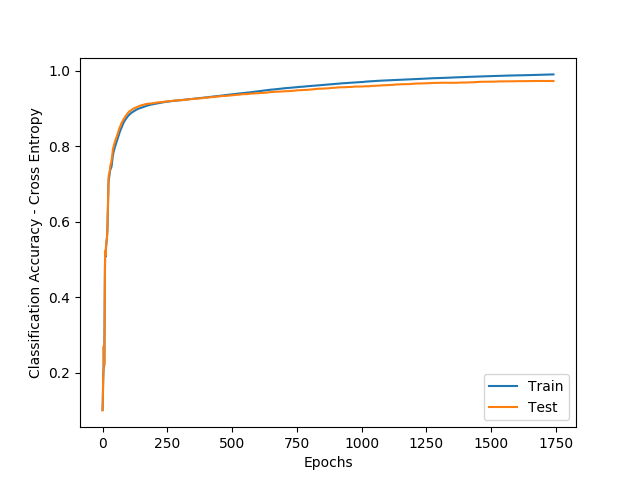
\includegraphics[width=9cm, height=6cm]{B4_c_1.png}
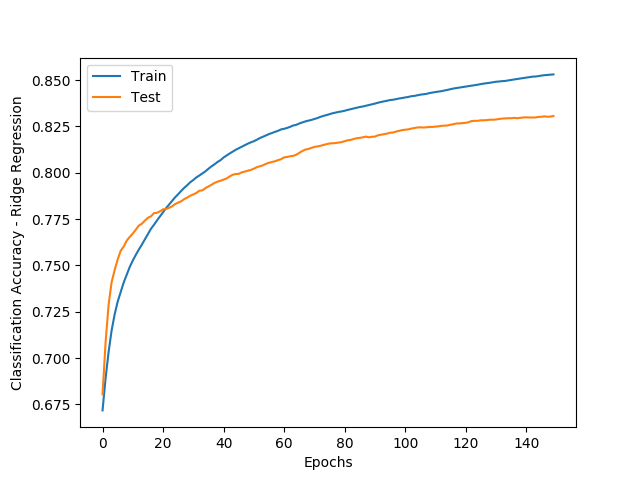
\includegraphics[width=9cm, height=6cm]{B4_c_2.png}


\begin{minted}[mathescape,linenos,obeytabs=true,tabsize=2]{python}

import torch
import numpy as np
import matplotlib.pyplot as plt
from mnist import MNIST

def load_data():
	mndata = MNIST('python-mnist/data/')
	X_train, labels_train = map(np.array, mndata.load_training())
	X_test, labels_test = map(np.array, mndata.load_testing())
	X_train = X_train / 255.0
	X_test = X_test / 255.0
	return X_train, labels_train, X_test, labels_test
X_train, y_train, X_test, y_test = load_data()

# One hot encoding
def one_hot(y_train_, m):
	n = len(y_train_)
	reformed_tensor = torch.zeros(n, m)
	for i in range(n):
		index = y_train_[i]
		reformed_tensor[i][index] = 1
	return reformed_tensor


# convert to tensor
X_train_ = torch.tensor(X_train, dtype=torch.double)
y_train_ = torch.tensor(y_train, dtype=torch.int64)

X_test_ = torch.tensor(X_test, dtype=torch.double)
y_test_ = torch.tensor(y_test, dtype=torch.int64)

W = torch.zeros(784, 10, requires_grad=True, dtype=torch.double)
W_mse = torch.zeros(784, 10, requires_grad=True, dtype=torch.double)
step_size = 0.01
epochs = 100
train_accuracy_list = []
test_accuracy_list = []
train_accuracy_list_mse = []
test_accuracy_list_mse = []

epochs = list(range(epochs))
for epoch in epochs:
	print("Epoch: ", epoch)
	y_hat = torch.matmul(X_train_, W)
	y_hat_mse = torch.matmul(X_train_, W_mse)
	# cross entropy combines softmax calculation with NLLLoss
	loss = torch.nn.functional.cross_entropy(y_hat, y_train_)
	loss_mse = torch.nn.functional.mse_loss(y_hat_mse, one_hot(y_train_, 10).double())
	# computes derivatives of the loss with respect to W
	loss.backward()
	loss_mse.backward()
	# gradient descent update
	W.data = W.data - step_size * W.grad
	W_mse.data = W_mse.data - step_size * W_mse.grad
	# .backward() accumulates gradients into W.grad instead
	# of overwriting, so we need to zero out the weights
	
	# Cross Entropy
	max_index_train = torch.max((torch.matmul(X_train_, W)), dim=1).indices.numpy()
	num_corrected_prediction_train = sum(max_index_train == y_train)
	train_accu = num_corrected_prediction_train / len(y_train)
	train_accuracy_list.append(train_accu)
	
	max_index_test = torch.max((torch.matmul(X_test_, W)), dim=1).indices.numpy()
	num_corrected_prediction_test = sum(max_index_test == y_test)
	test_accu = num_corrected_prediction_test / len(y_test)
	test_accuracy_list.append(test_accu)
	
	# MSE
	max_index_train_mse = torch.max((torch.matmul(X_train_, W_mse)), dim=1).indices.numpy()
	num_corrected_prediction_train_mse = sum(max_index_train_mse == y_train)
	train_accu_mse = num_corrected_prediction_train / len(y_train)
	train_accuracy_list_mse.append(train_accu_mse)
	
	max_index_test_mse = torch.max(torch.matmul(X_test_, W_mse), dim=1).indices.numpy()
	num_corrected_prediction_test_mse = sum(max_index_test_mse == y_test)
	test_accu_mse = num_corrected_prediction_test_mse / len(y_test)
	test_accuracy_list_mse.append(test_accu_mse)
	
	
	
	print("Train Accuracy: ", train_accu)
	print("Test Accuracy: ", test_accu)
	
	W.grad.zero_()
	W_mse.grad.zero_()

plt.plot(epochs, train_accuracy_list, label="Train")
plt.plot(epochs, test_accuracy_list, label="Test")
plt.xlabel("Epochs")
plt.ylabel("Classification Accuracy - Cross Entropy")
plt.legend()
plt.savefig("/Users/yinruideng/Desktop/senior_spring/cse546/hw/hw2/latex/B4_c_1.png")
plt.show()

plt.plot(epochs, train_accuracy_list_mse, label="Train")
plt.plot(epochs, test_accuracy_list_mse, label="Test")
plt.xlabel("Epochs")
plt.ylabel("Classification Accuracy - Ridge Regression")
plt.legend()
plt.savefig("/Users/yinruideng/Desktop/senior_spring/cse546/hw/hw2/latex/B4_c_2.png")
plt.show()
\end{minted}







\end{document}